\documentclass[english, 10pt]{article}
\usepackage[sexy]{evan}
\usepackage{inconsolata}
\usepackage[shellescape]{gmp}
\usepackage{titlesec}
\usepackage{color}
\usepackage{logicproof}
\usetikzlibrary{arrows.meta}
\definecolor{editorGray}{rgb}{0.95, 0.95, 0.95}
\definecolor{editorOcher}{rgb}{1, 0.5, 0} % #FF7F00 -> rgb(239, 169, 0)
\definecolor{editorGreen}{rgb}{0, 0.5, 0} % #007C00 -> rgb(0, 124, 0)
\usepackage{listings}
\usepackage{xcolor}
\usepackage[toc,page]{appendix}
\usepackage{todonotes}
\usepackage{blindtext}
\usepackage{multicol}
\usetikzlibrary{calc,shapes.multipart,chains,arrows}
\usepackage{esint}
\usetikzlibrary{shapes.multipart}


\definecolor{dkgreen}{rgb}{0,0.6,0}
\definecolor{gray}{rgb}{0.5,0.5,0.5}
\definecolor{mauve}{rgb}{0.58,0,0.82}

\lstset{frame=tb,
  language=Java,
  aboveskip=3mm,
  belowskip=3mm,
  showstringspaces=false,
  columns=flexible,
  basicstyle={\small\ttfamily},
  numbers=none,
  numberstyle=\tiny\color{gray},
  keywordstyle=\color{blue},
  commentstyle=\color{dkgreen},
  stringstyle=\color{mauve},
  breaklines=true,
  breakatwhitespace=true,
  tabsize=3
}

\allowdisplaybreaks%
\renewcommand{\O}{\mathcal{O}}
\newcommand{\thiscoursecode}{CMSC 250}
\newcommand{\thiscoursename}{Discrete Mathematics}
\newcommand{\thisprof}{Prof. Mohammad Nayeem Teli}
\newcommand{\me}{Axel Balestrieri}
\author{Axel Balestrieri\thanks{Email: \mailto{axelb2004@icloud.com}}}
\newcommand{\thisterm}{Fall 2023}
\newcommand{\website}{https://www.cs.umd.edu/class/fall2023/cmsc250-020X/}%chktex 8
\usepackage{ifpdf}
\ifpdf%
\DeclareGraphicsRule{*}{mps}{*}{}
\fi
\lhead{\textbf{\me} \\ \textbf{\thisprof}}
\rhead{\textbf{\thiscoursename} \\ \textbf{\thisterm}}

\newcommand{\notefront}{%
\pagenumbering{arabic}
\begin{center}
{\small}
\textbf{\Huge{{\thiscoursecode}}}
{\Huge \par}
{\Large{{\thiscoursename}}}\\
\vspace{0.1in}
\vspace{0in}
\includegraphics[scale=0.3]{media/cs.jpg} \\
\vspace{0.1in}{\me} \\
{\thisprof} \ $\bullet$ \ {\thisterm} \ $\bullet$ \ {{University of Maryland}} \\
{\ttfamily \url{\website}} \\
\end{center}
}

\begin{document}
  \thispagestyle{empty}
  \notefront
  \tocandfigures

\section{Tuesday, August 29, 2023}
Welcome to CMSC250, also known as Discrete Structures through UMD. In this class, we will go over logic and its statements, and eventually lead up to being able to write formal, elegant proofs.

\subsection{DISCLAIMER}
The notes written in this document do NOT fully cover the entirety of CMSC250, as some examples may have been omitted for simplicity. All examples and worksheets can be found online for extra practice (do use them, this information is very general!) For extra notes and examples, visit:\\
https://www.math.umd.edu/(tilde)immortal/CMSC250/.

\subsection{Statements and Logic}
In discrete mathematics, we like to introduce ourselves to the idea of how we may use \vocab{statements} to form logical expressions. In our class, a statement is \textbf{a proposition which can either hold a conclusion of it being true or false, but NEVER both.}

Lets look at a few examples, and try to distinct if they are statements or not.

\begin{example}
    Statement or not?
    3 + 3 = 6
\end{example}

This is quite intuitive, but this is of course, a statement, as we know commonly that 3 plus 3 really does equal 6, therefore giving making it true.

How about this one?

\begin{example}
    Statement or not?
    \(x > 20\).
\end{example}

Now, you may say, this can be a statement because we can just make \(x\) a value either greater than or less than 20, and it will either be true or false! Well... no. Since the value can differ between either true or false, and we do not EXPLICITLY know what \(x\) is, this is not a statement.

\subsection{Logical Negation, Disjunction, Conjunction, XOR, and Precedence}
In common logic, we use different variables to represent statements called \vocab{statement variables}. Typically, these statement variables will be denoted by using letters starting from \(p\), then going to \(q\), and et cetera.

\subsubsection{Negation (Not)}
\textbf{\underline{Definition 1.1}}: Suppose we are given some statement or statement variable \(p\). Given this, we can interpret the negation of \(p\) to be "not \(p\)", or the opposite of \(p\). Writing this out for logic problems, we use the symbol \neg{p}.

\subsubsection{Disjunction (Or)}
\textbf{\underline{Definition 1.2}}:  Given two propositions, \(p\) and \(q\), such that \(p\) is not equal to \(q\), we now know \(p\)\lor\(q\) is true if all or either value is true.

\subsubsection{Conjunction (And)}
\textbf{\underline{Definition 1.3}}: Given two propositions, \(p\) and \(q\), such that \(p\) is equal to \(q\), we now know $p\land q$ is true if and only if both values are true.

\subsubsection{XOR $(\oplus)$}
\textbf{\underline{Definition 1.4}}: XOR (exclusive or) can be considered one or the other, but not the same as or in logic. Also known as being true if either \(p\) is true or \(q\) is true, but never both.

\subsubsection{Precedence}
\begin{itemize}
    \item Conjunction and disjunction have equal precedence.
    \item Negation has first precedence.
    \item Considering the statement, XOR may have equal precedence to disjunction, or it may not.
\end{itemize}

\subsubsection{Interpretations and Translating Statements}
In logic examples, it is common to have to translate English sentences into logical statements (you will see this on quizzes and exams!). Let's look at a few examples.

\begin{example}
    I am hungry or I am tired.
\end{example}

In this example, let \(p\) be "I am hungry," and \(q\) be "I am tired." From this, we can get the answer: $p\lor q.$\\

\begin{example}
    Either I am hilarious or you have no sense of humor.
\end{example}

In this example, let \(p\) be "I am hilarious," and \(q\) be "You have a sense of humor." From this, we can get the answer: $p \oplus \neg{q}$\\


\subsection{Truth Tables}
In logic, we like to portray truth values (either when \(p\) is true or false) in a table called the \vocab{truth table}. This allows us to easily interpret different outcomes if we give our statement variables alternating values.
\begin{example}
Fill in the truth table for the values with question marks.
\begin{displaymath}
\begin{array}{|c c|c|c|}
% |c c|c| means that there are three columns in the table and
% a vertical bar ’|’ will be printed on the left and right borders,
% and between the second and the third columns.
% The letter ’c’ means the value will be centered within the column,
% letter ’l’, left-aligned, and ’r’, right-aligned.
p & q & p \land q & p \lor q\\ % Use & to separate the columns
\hline % Put a horizontal line between the table header and the rest.
T & T & ? & ?\\
T & F & ? & ?\\
F & T & ? & ?\\
F & F & ? & ?\\
\end{array}
\end{displaymath}
\end{example}


Using our definitions of disjunction and conjunction, we can fill out the truth table to look like this now:

\begin{displaymath}
\begin{array}{|c c|c|c|}
% |c c|c| means that there are three columns in the table and
% a vertical bar ’|’ will be printed on the left and right borders,
% and between the second and the third columns.
% The letter ’c’ means the value will be centered within the column,
% letter ’l’, left-aligned, and ’r’, right-aligned.
p & q & p \land q & p \lor q\\ % Use & to separate the columns
\hline % Put a horizontal line between the table header and the rest.
T & T & T & T\\
T & F & F & T\\
F & T & F & T\\
F & F & F & F\\
\end{array}
\end{displaymath}

Lets look at another example (this one is quite useful!)

\begin{example}
    Finish the truth table below, indicating every step to reach the final value.
    \begin{displaymath}
    \begin{array}{|c c|c|}
    p & q & (p \lor q)\land \neg{(p \land q)}\\ 
    \hline
    F & F & ?\\
    F & T & ?\\
    T & F & ?\\
    T & T & ?\\
    \end{array}
    \end{displaymath}
\end{example}

Combining our definitions of negations, disjunctions, and conjunctions, we can reach a final truth table that looks something like this:

\begin{displaymath}
    \begin{array}{|c c|c|c|c|}
    p & q & p \lor q & p \land q &(p \lor q)\land \neg{(p \land q)}\\ 
    \hline
    F & F & F & F & F\\
    F & T & T & F & T\\
    T & F & T & F & T\\
    T & T & T & T & F\\
    \end{array}
    \end{displaymath}

If we look very closely to our final value, we have essentially proved the XOR operator! (This'll come in handy when logical equivalence becomes more prevalent.)

\section{Thursday, August 31, 2023}
\subsection{Logical Equivalence}
In logic, when we say that two statements show the same T/F value for every possible combination of component statement variables, we like to consider those two statements \vocab{logically equivalent}. This is commonly denoted through the "\equiv" symbol.

\begin{example}
    Is the following logically equivalent? \(p\) and \neg{(\neg{p})}
\end{example}

This example is very, very elementary, but let's just show it through a truth table in case you're scratching your head at it.

\begin{displaymath}
    \begin{array}{|c|c|c|}
    p & \neg{p} & \neg{(\neg{p})}\\ 
    \hline
    T & F & T\\
    F & T & F\\
    \end{array}
\end{displaymath}

Through this truth table, now we see that the first column is directly equivalent to the last column for any value, so: \(p\) \equiv \neg{(\neg{p})}.

This is considered the \vocab{double negative}.

\subsection{DeMorgan's Laws}
In logical equivalence, there are two laws that will be extensively used called \vocab{DeMorgan's laws}. These cover two very important logical equivalencies.

\begin{displaymath}
    \neg{(p \lor q)}\equiv \neg{p} \land \neg{q}
\end{displaymath}

\begin{displaymath}
    \neg{(p \land q)}\equiv \neg{p} \lor \neg{q}
\end{displaymath}
 
We can use these two laws when we prove logical equivalency to hasten our final conclusion.

\subsection{Tautologies and Contradictions}
\vocab{Tautologies} are a form of statement in which the statement form is \textbf{true} for all values, no matter true nor false.

Say for example, we have \(x\) as a tautology. Therefore, we can simply write:

\begin{displaymath}
    x = t
\end{displaymath}

\begin{example}
    An elementary tautology is $p \land \neg{p}$.
\end{example}

\vocab{Contradictions}, on the other hand, are a form of statement in which the statement form is \textbf{false} for all values, no matter true nor false.

Say for example, we now have \(y\) being a contradiction. Therefore, we can simply write:

\begin{displaymath}
    y = c
\end{displaymath}

\begin{example}
    An elementary contradiction is $p \lor \neg{p}$.
\end{example}

\subsection{Condensing and Proving Logical Equivalencies}
Over time, many particular logical equivalencies have been created, to a point where we can consider them as generalized laws that we may use to help in our steps to prove logical equivalencies that have not been proven. We call these the \vocab{common logical equivalencies} as demonstrated in the table below.

\vspace{0in}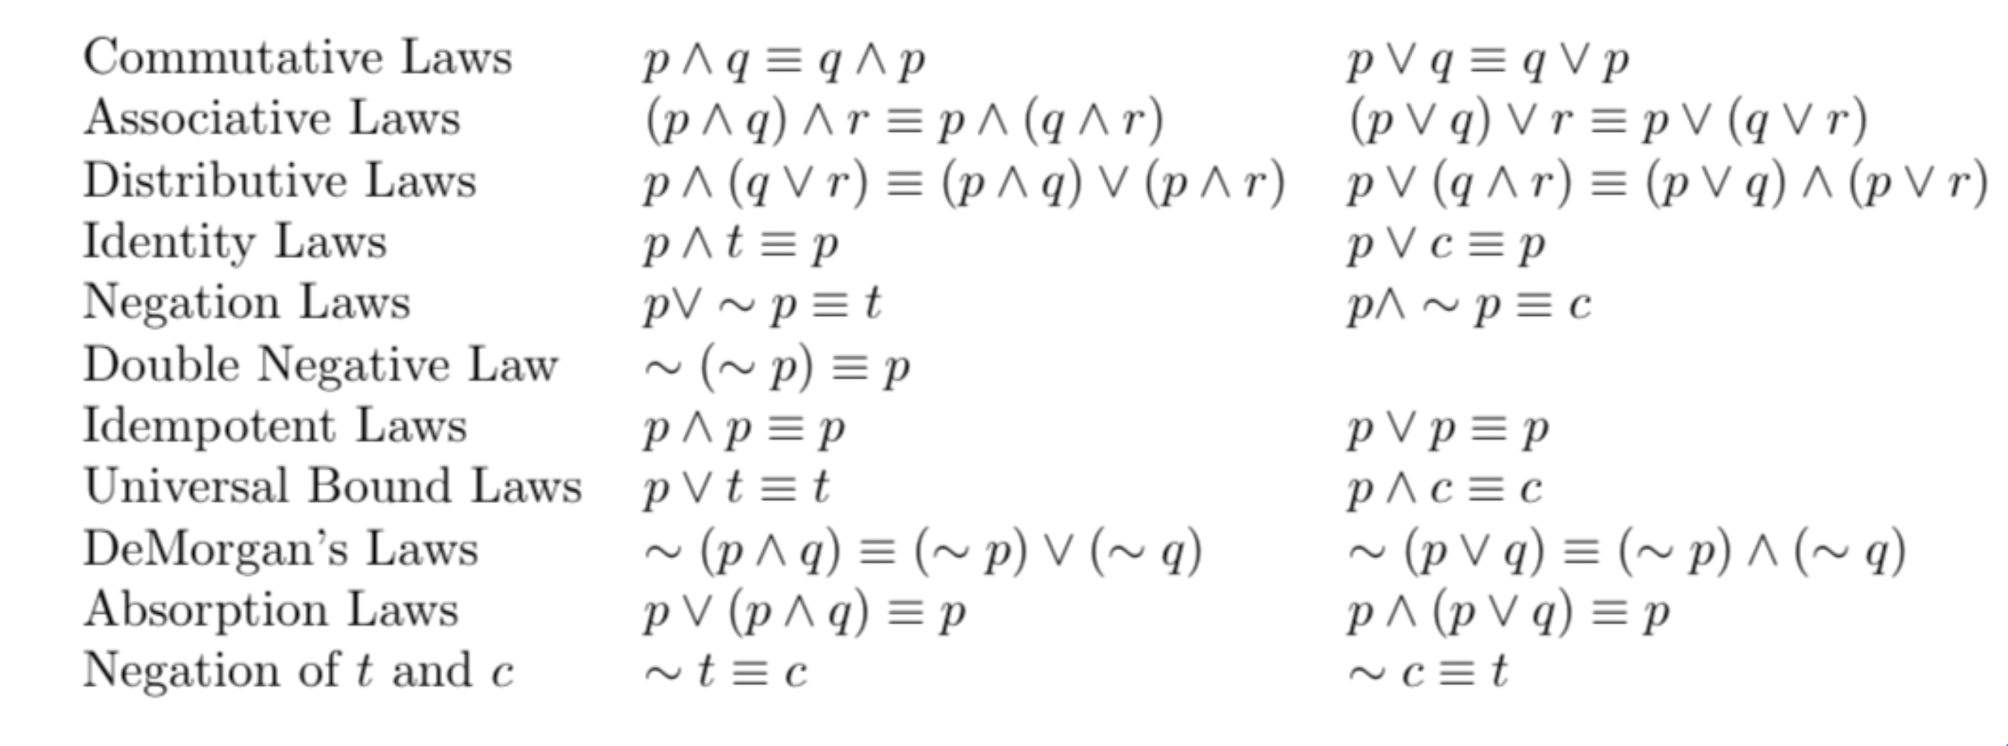
\includegraphics[scale=0.4]{media/commonlogicalequivalencies.png} \\

Lets use these laws to prove some logical equivalencies ourselves.

\begin{example}
    Prove $\neg(\neg p\land q)\land(p\lor q)\equiv p.$
\end{example}

Using the table above, this would be the proof (there can be other solutions!) to this example.
\begin{logicproof}{1}
    \neg{(\neg{p}\land q)\land(p\lor q)} & Original Left Side \\
    (\neg({\neg{p})}\lor \neg{q})\land (p\lor q) & DeMorgan's Law \\
    (p\lor \neg{q}) \land (p\lor q) & Double Negative Law \\
    p \lor (\neg{q}\land q) & Distributive Law \\
    p \lor c & Negation Law \\
    p & Identity Law
\end{logicproof}

\subsection{Conditional Statements}
In logic, we can also consider implications of statements such like "if \(p\), then \(q\)." These are considered \vocab{conditional statements}, and they too can be treated as ordinary logic signs (there is also a logical equivalency for implications and normal logic signs).

Say we have statement variables \(p\) and \(q\). We can then derive a conditional form:

\begin{displaymath}
    p \rightarrow q
\end{displaymath}

The general idea for implication is that if we have \(p\) being true and \(q\) being false, then the implication is then false. However, otherwise the implication is always true.

The logical equivalence of the normal conditional is:

\begin{displaymath}
    p \rightarrow q \equiv \neg p \lor q
\end{displaymath}

This can be written in logical equivalence proofs by just indicating that this is the "definition of implication" or "definition of conditional."
\section{Tuesday, September 5, 2023}

\subsection{More on Conditional Statements}
With conditional statements, we can expand them into different archetypes to create more basis for logical equivalencies. We call these the \vocab{converse, inverse, }and \vocab{contrapositive}.

\subsubsection{Converse}
The converse of a logical statement is more or less just re-arranging the statement variables so that they are reversed. Therefore, the converse of a statement:
\begin{displaymath}
    p \rightarrow q
\end{displaymath}
is expressed as:
\begin{displaymath}
    q \rightarrow p
\end{displaymath}

Of course, from this it would be pretty intuitive to say that the converse is \textbf{not} logically equivalent to the original statement.

\subsubsection{Contrapositive}
The contrapositive of a logical statement is practically just the negation of a converse, or using DeMorgan's law (only on the statement variables) of the converse. Therefore, the contrapositive of a logical statement is:
\begin{displaymath}
    p \rightarrow q
\end{displaymath}
is expressed as:
\begin{displaymath}
    \neg q \rightarrow \neg p
\end{displaymath}

This would mean that the original statement and the contrapositive of that statement \textbf{are} logically equivalent.

\subsubsection{Inverse}
The inverse of a logical statement is the negation of the original statement itself. Therefore, the inverse of a logical statement can be shown as:
\begin{displaymath}
    p \rightarrow q
\end{displaymath}
being:
\begin{displaymath}
    \neg p \rightarrow \neg q
\end{displaymath}

\subsection{Biconditionals}
In logic, we can treat implications where it can be described as an "if any only if" statement as a \vocab{biconditional}. Portrayed through the truth table, we can see:

\begin{displaymath}
    \begin{array}{|c|c|c|}
    p & q & p \iff q\\ 
    \hline
    T & T & T\\
    T & F & F\\
    F & T & F\\
    F & F & T\\
    \end{array}
\end{displaymath}

The biconditional also has its own logical equivalence, considering it the tautology:

\begin{displaymath}
    p \iff q \equiv (p \rightarrow q) \land (q \rightarrow p)
\end{displaymath}

\subsubsection{Necessary and Sufficient Conditions}
Suppose we have statements p and q in a biconditional. We can distinguish two different conditions for p and q depending on how the whole statement is written.

\begin{itemize}
    \item p is a sufficient condition for q means, if p then q.
    \item p is a necessary condition for q means if not p then not q.
\end{itemize}

\subsection{Arguments and Rules of Inference}
\textbf{\underline{Definition 3.1}}: An \vocab{argument} is a conjecture that say that if you make certain assumptions, then a particular statement must follow.

\begin{itemize}
    \item The assumptions are called \vocab{premises}.
    \item The statement that follows is the \vocab{conclusion.}
\end{itemize}

An argument is considered valid when, for all interpretations that make the premises true, the conclusion is also true.

Recall the laws of logical equivalencies.

\vspace{0in}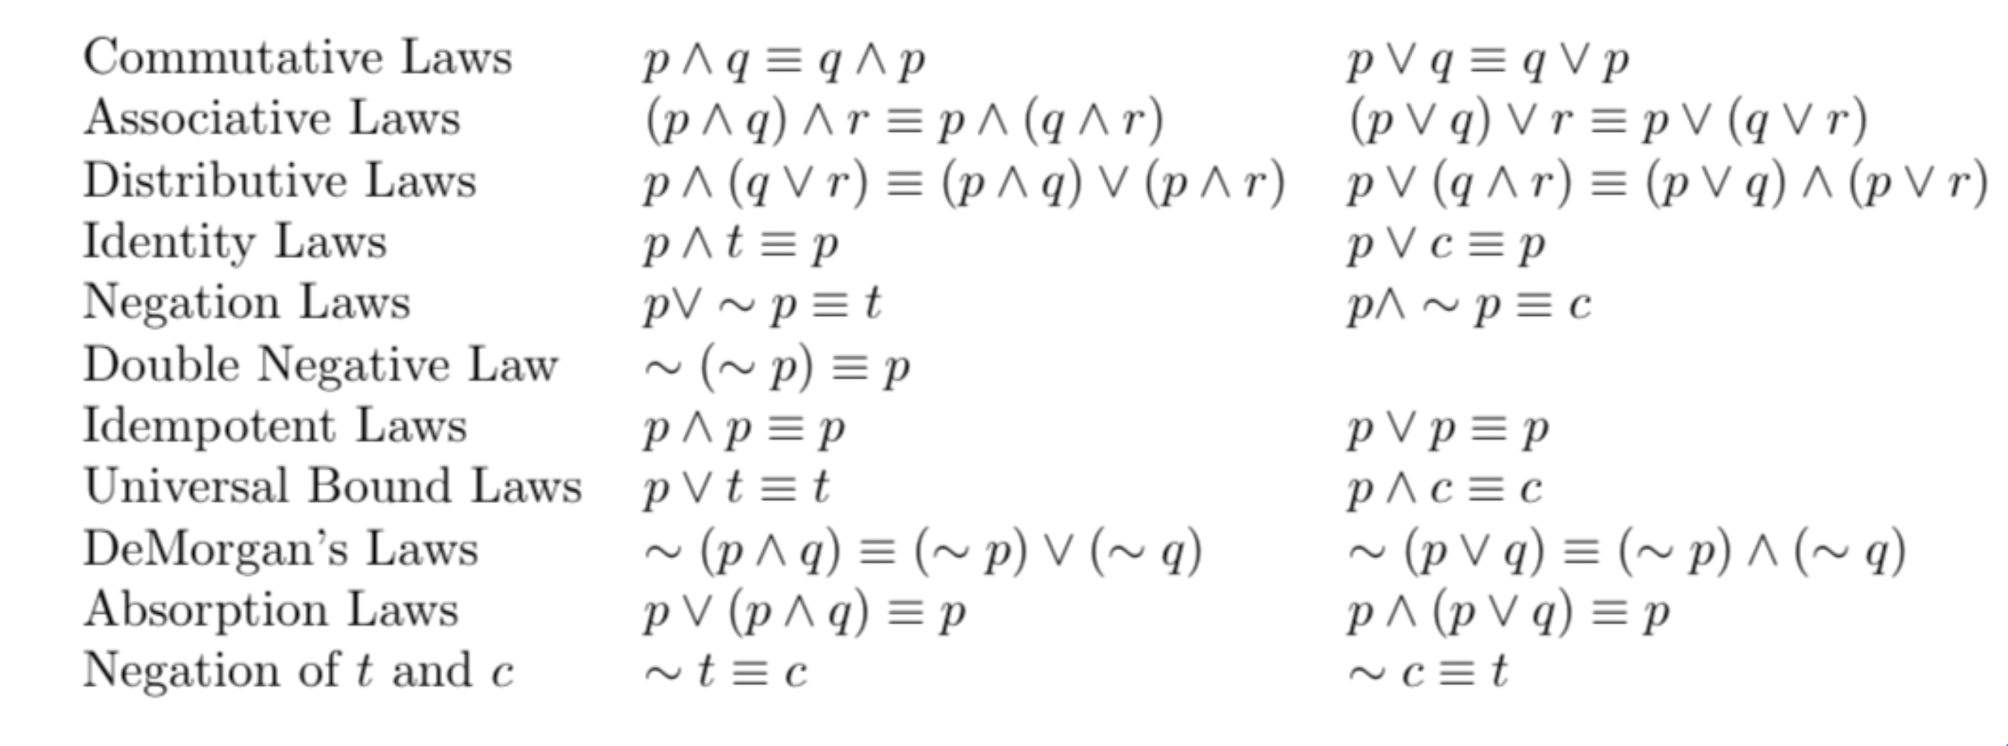
\includegraphics[scale=0.4]{media/commonlogicalequivalencies.png} 

We can use these in proving arguments, alongside our new friend, the \vocab{rules of inference}. We can use these rules of inference to prove the validity of complex arguments.

\vspace{0in}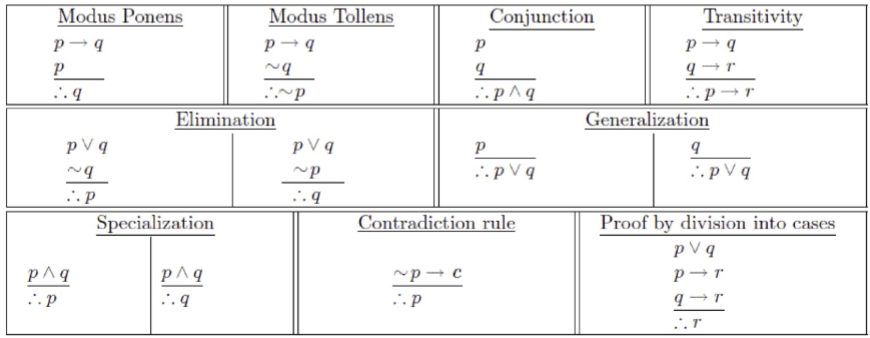
\includegraphics[scale=1]{media/Screenshot 2023-10-02 at 5.51.13 PM.png} 

\begin{example}
$p \iff q$\\
$q \rightarrow r$\\
$p \lor s$\\
$\neg r$\\
$\therefore s$
\end{example}

Using logical equivalence and rules of inference, we can prove this pretty easily.

\begin{logicproof}{1}
p \iff q & Premise\\
q \rightarrow r & Premise\\
p \lor s & Premise\\
\neg r & Premise\\
(p \rightarrow q) \land (q \rightarrow p) & Definition of Biconditional of 1\\
p \rightarrow q & Specialization of 5\\
q \rightarrow p & Specialization of 5\\
p \rightarrow r & Transitivity of 2 and 7\\
\neg p & Modus Tollens of 8 and 4\\
s & Elimination of 3 and 9
\end{logicproof}
\section{Thursday, September 7, 2023}

\subsection{Number Bases}
All numbers contain the same concept between each other, called their \vocab{number base}. The number base, in short, is the number of digits that a system of counting uses to represent numbers. For example, if we have a number in base 10, 639, the 9 is in ones place, 3 is in the tens place, and 6 is in the hundreds place.

In this course, we will be focusing on decimal and binary numbers.

\subsubsection{Decimal (Base 10)}
\textbf{\underline{Definition 4.1:}} A decimal number has the expression:

\begin{displaymath}
    n : ...d_3d_2d_1d_0
\end{displaymath}

Therefore..

\begin{displaymath}
    n_1_0 = ... + d_3 * 10^3 + d_2 * 10^2 + d_1 * 10^1 + d_0 * 10^0
\end{displaymath}

\subsubsection{Binary (Base 2)}
\textbf{\underline{Definition 4.2:}} A binary number has the expression:

\begin{displaymath}
    n : ...d_3d_2d_1d_0
\end{displaymath}

Therefore..

\begin{displaymath}
    n_1_0 = ... + d_3 * 2^3 + d_2 * 2^2 + d_1 * 2^1 + d_0 * 2^0
\end{displaymath}

\subsection{Converting from Binary to Decimal, and Decimal to Binary}
Converting from binary to decimal is straightforward, as all you need to do is use the formula given above and you will get your base 10 number. However, for decimal to binary, you must:

\begin{logicproof}{1}
     & Divide the given decimal number by 2 constantly (Divide each quotient until 0). \\
     & Gather all remainders from the division (either 1 or 0). \\
     & Starting from the last remainder to the first remainder, build your new binary  number.
\end{logicproof}

\subsection{Digital Circuits}
\textit{Look online through Justin's notes on digital circuits, as drawings must be made.}
\section{Tuesday, September 12, 2023}
\subsection{Propositional Logic: Are we being limited?}
All the logic we have already discussed in class all had to revolve around propositions and their logic. However, only using propositions limits our capabilities to what we can and can't have defined at once. For example:

\begin{center}
    All men are mortal \\
    Socrates is a man \\
    $\therefore$ Socrates is a mortal.
\end{center}

The statement logic here is circumscribed by the variables we give it. "All men are mortal" is a good example here. What if we just have some man, not all? This is where \vocab{predicates} can come into play, and make our jobs easier.

\subsection{Predicates}
\textbf{\underline{Definition 5.1}}: A predicate is a sentence containing variables. To obtain a predicate, we can remove one or more nouns.

\begin{example}
    The sentence "\(x\) is greater than 3" has two parts.\\
    The first part, \(x\) is the subject. \\
    The second part, "is greater than 3" is considered the predicate.
\end{example}

With predicates, we typically assign different predicate symbols: 1. the predicate itself, and 2. the domain, or the set that the predicate variable belongs to.

\begin{example}
    Predicate: \(Q(x\)) such that \(x\) is even. \\
    Domain: \(x\) \in \mathbb{Z}
\end{example}

\subsection{Predicates with Logical Connectives}
The common logical connectives we've used (OR, AND, XOR) can be used to join predicates to make more complex predicates.

\begin{example}
    \begin{displaymath}
    T(x,y) = (A(x) \land G(x,y)) \rightarrow \neg L(y)
    \end{displaymath}
    \begin{center}
        another example being...
    \end{center}
    \begin{displaymath}
        P(x) = \neg Q(x) \lor R(x)
    \end{displaymath}
\end{example}

\subsection{Quantifiers}
So far, we've been able to figure out the truth or falsehood of statements that include variables. However, what if we expand out to see if it applies to all values in that domain, or only some? This is when we bind our variables using \vocab{quantifiers}.

\subsubsection{The Universal Quantifier}
\textbf{\underline{Definition 5.2}}: The universal quantifier "for all" $(\forall)$, says that a statement MUST be true for all values of that variable.

\begin{example}
    All humans are mortal.\\
    $\forall x$: Human(x) $\rightarrow$ Mortal(x)
\end{example}

To make the universal value explicit, we use the set notation ($\in$). Also, universal quantifiers are logically equivalent to if we put the predicate into an infinite AND connector.

\begin{example}
    $\forall x \in \mathbb{N} : P(x)$\\
    $P(0) \land P(1) \land P(2) \land $ ...
\end{example}

\subsubsection{The Existential Quantifier}
\textbf{\underline{Definition 5.3}}: The existential quantifier "there exists" $(\exists)$, says that a statement MUST be true for at LEAST one value of the variable.

\begin{example}
    There is a student is CMSC250.\\
    $\exists x \in P$: x is a student in CMSC250 where P is the set of all people. 
\end{example}

\subsection{Negations of Quantifiers}
Remember DeMorgan's laws? Well, they can also apply to quantifiers almost identically to how they applied to connectors in propositional logic. The following equivalencies hold:

\begin{center}
    $\neg \forall x: P(x) \equiv \exists x: \neg P(x)$\\
    $\neg \exists x: P(x) \equiv \forall x: \neg P(x)$
\end{center}

These are the quantifier versions of DeMorgan's laws.

\begin{example}
    \textbf{What would the negation of this be?}\\
    Every Student in your class has taken a course in Calculus.\\
    $\forall x P(x)$\\
    P(x) is the statement "x has taken a course in calculus" and $x \in $ students.
\end{example}

The negation of this statement would be "It is not the case that every student in your class has taken a course in calculus." This is also equivalent to "There is a student in your class who has not taken a course in calculus."

Do \textbf{NOT} use "none" to negate "every"!!! This is not logically equivalent, as the negation of "every" is "some".

\subsection{An Intro to Nested Quantifiers}
Quantifiers can also be nested, since predicates can take in more than one variable. Keep in mind that the order of which variable goes where DOES matter, as they may not be logically equivalent in scenarios. See the table for more.\\

\begin{center}
    \vspace{0in}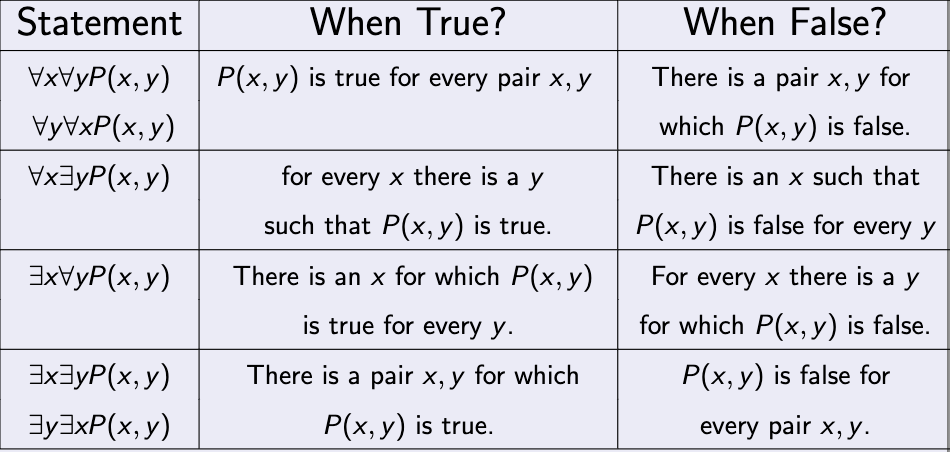
\includegraphics[scale=.7]{media/table.png} \\
\end{center}

\section{Thursday, September 14, 2023}
\subsection{More on Predicate Logic: Truth and Falsity}
For universal and existential quantifiers, it is imperative that we establish how to find if an existential and/or universal statement is true or false.

\begin{itemize}
    \item To show $\exists$ statement is true, find an example in the domain where it is true.
    \item To show $\exists$ statement is false, show false for every member of the domain.
    \item To show $\forall$ statement is true, show true for every member of the domain.
    \item To show $\forall$ statement is false, find an example in the domain where it is false.
\end{itemize}

Do note that the domain does matter!

\begin{example}
\textbf{Is the following true:}\\
$\forall x \exists y: y<x$
\end{example}

To determine whether or not this is true, we must establish:
\begin{itemize}
    \item Is the domain $\mathbb{N}$? (Naturals)
    \item Is the domain $\mathbb{Z}$? (Integers)
    \item Is the domain $\mathbb{Q}$? (Rationals)
    \item Is the domain $\mathbb{Q}^>^0$? (Rationals that are greater than 0)
    \item Is the domain $\mathbb{Q}^>^=^0$? (Rationals that are greater than or equal to 0)
    \item Is the domain $\mathbb{R}$? (Reals)
    \item Is the domain $\mathbb{C}$? (Complex)
\end{itemize}

\subsection{Vacuity in Universal Statements}
\textbf{\underline{Definition 6.1}}: If domain, D, is empty, then $(\exists x \in D)[P(x)]$ is vacuously false. This then means that if domain, D, is empty, then $(\forall x \in D)[P(x)]$ is vacuously true.

\begin{example}
    All balls in the bowl are blue. \textbf{Is it true or false?}
\end{example}

This statement is false, if and only if, its negative is true. Its negation is "there exists a ball in the bowl that is not blue." But what if the bowl is empty?

If the bowl is empty, the negation would then be false as there does not exist a ball in the bowl that is not blue, which makes the original statement true by "default" or in other words, vacuously true.

\subsection{Order Matters}
The order for which domain values variables are placed in a predicate statement do indeed matter.

\begin{example}
    $Q(x,y,z): x+y=z$, for $x,y,z \in \mathbb{R}$\\
    \textbf{Are these statements equivalent?}\\
    $\forall x \forall y \exists z: Q(x,y,z)$\\
    $\exists z \forall x \forall y: Q(x,y,z)$
\end{example}

\textbf{Try to do this one yourself :)}

\subsection{Negating Nested Quantifiers}
Negation of quantifiers works exactly like how one would expect it to work, just like De Morgan's laws.

\begin{example}
    \textbf{Express the negation of the statement: }$\forall x \exists y: (xy=1)$ 
\end{example}

As typical, apply De Morgan's laws carefully and then you will get the final answer.

\begin{center}
    $\exists x \neg \exists y: (xy=1)$\\
    $\exists x \forall y: \neg (xy=1)$\\
    $\exists x \forall y: (xy\neq 1)$
\end{center}
\section{Tuesday, September 19, 2023}
\subsection{Extending our Rules of Inference}
\subsubsection{Universal Instantiation}
\textbf{\underline{Definition 7.1:}} We conclude that $P(c)$ is true, where \(c\) is a particular member of the domain, given the premise $\forall xP(x)$.

\begin{example}
Given Marvin $\in$ Martians:\\
All Martians are green\\
$\therefore$ Marvin is green.
\end{example}

To show this in formal logic proof, we can show universal instantiation to be shown like:

\begin{center}
    $\forall x \in D[P(x)]$\\
    $\therefore P(c)$, for any $c\in D$.
\end{center}

\subsubsection{Universal Generalization}
\textbf{\underline{Definition 7.2:}} We conclude that $\forall xP(x)$ is true, given the premise that $P(c)$ is true for all elements \(c\) in the domain. The element \(c\) must be an arbitrary, and not a specific element of the domain.

\begin{example}
    $P(c): c \geq 0$\\
    $c \in \mathbb{N}[P(c)]$\\
    $\therefore \forall x \in \mathbb{N}[P(x)]$
\end{example}

To show this in formal logic proof, we can show universal generalization to be shown like:

\begin{center}
    $P(c)$, for some $c \in D$ (selected arbitrarily)\\
    $\therefore \forall x \in D[P(x)]$
\end{center}

\subsubsection{Existential Instantiation}
\textbf{\underline{Definition 7.3:}} Suppose we know that $\exists x: P(x)$ is true. We can then conclude that there is an element c in the domain for which $P(c)$ is true.

To show this in formal logic proof, we can show existential instantiation to be shown like:

\begin{center}
    $\exists x \in D[P(x)]$\\
    $\therefore P(c)$ for some element $c \in D$
\end{center}

\subsubsection{Existential Generalization}
\textbf{\underline{Definition 7.4:}} Suppose that for a particular element c, if we know $P(c)$ is true, we can conclude that $\exists x P(x)$ is true.

To show this in formal logic proof, we can show existential generalization to be shown like:

\begin{center}
    $P(c)$ for some $c \in D$\\
    $\therefore \exists x \in D[P(x)]$
\end{center}

\subsection{Proofs}
Proofs are the deductive arguments for a mathematical statement, which shows the stated assumptuons which logically guarantee the conclusion. In common proof, they are made up of multiple different parts which in the end, add up to be all one body.

With proof, we have different terminologies.

\begin{itemize}
    \item A \vocab{theorem} is a statement that can be shown to be true.
    \item A \vocab{lemma} is a less important theorem that is helpful in the proof of other results.
    \item A \vocab{corollary} is a theorem that can be established directly from a theorem that has been proved.
    \item A \vocab{conjecture} is a statement that is being proposed to be a true statement.
    \item A \vocab{proof} is a valid argument that establishes the truth of a theorem.
    \item An \vocab{axiom} is a statement we assume to be true.
\end{itemize}

A good proof usually has:

\begin{itemize}
    \item A clear statement of what is to be proved (labelled as theorem, lemma, proposition, or corollary).
    \item The word "Proof" to indicate where the proof starts.
    \item A clear indication of flow.
    \item A clear justification for each step.
    \item A clear indication of the conclusion.
    \item The abbreviation "QED" or $\blacksquare$ to indicate the end of the proof.
\end{itemize}

There are different kinds of proof methods that we may use to prove some statement, and depending on the question you are doing one proof method may be easier than the other (or might one not be feasible!) The different types of proof methods we use are

\begin{itemize}
    \item Direct proof
    \item Proof by contraposition
    \item Proof by contradiction
    \item Exhaustive proof
    \item Proof by cases.
\end{itemize}

\subsection{Statement of Theorems}
Know that for all of these, everything is equivalent (you can use these in your proofs!)

\begin{itemize}
    \item The sum of two positive integers is positive.
    \item If m, n are positive integers then their sum m + n is a positive integer.
    \item For all positive integers m, n their sum m + n is a positive integer.
    \item $(\forall m,n \in \mathbb{Z}) : [((m > 0)\land (n > 0)) \rightarrow ((m+n)>0)]$
\end{itemize}

\subsection{Definition of Numbers}
All numbers used in proof will have their own definitions in order to make our proofs a lot easier instead of having to rigorously prove why it is.

\textbf{\underline{Definition 7.3}}: An integer n is even if $n=2k$ or some integer k, and is odd if $n=2k+1$ for some integer k.

\textbf{\underline{Definition 7.4}}: A number q is rational if there exists integers a, b with $b \neq 0$ such that $q = a/b$.

\textbf{\underline{Definition 7.5}}: A real number that is not rational is irrational.

\subsubsection{Extra Closure of Definitions}
\begin{itemize}
    \item $\mathbb{Z}$ is closed under addition (If $a,b \in \mathbb{Z}$, then $a+b \in \mathbb{Z}$).
    \item $\mathbb{Q}^\neq^0$ is closed under division.
    \item $\mathbb{Z}^\neq^0$ is not closed under division.
\end{itemize}

Understand that closure practically means that if we add, subtract, multiply, or divide by two of the same type of number (i.e. $a,b \in \mathbb{Z} \rightarrow a+b \in \mathbb{Z}$), it will come out as that same type. Understand that for cases where we are trying to divide, some types of numbers that include 0 are not closed under division (i.e. $\mathbb{R}$, since reals contain 0 in their domain, and if $a,b \in \mathbb{R}$, there is a possibility that $a/b$ will be undefined.)

\subsection{Direct Proofs}
Let's go over some examples of direct proofs.

\begin{example}
    \textbf{Theorem: The square of an even number is even.}
\end{example}

\begin{proof}
Let $x = 2k$, where $k \in \mathbb{Z}$ by the definition of even numbers. Squaring both sides will give us $x^2=4k^2=2(2k^2)$. Let $m=2k^2$, where $m\in \mathbb{Z}$. $\therefore x^2=2m$, and by the definition of even numbers $x^2$ is even. QED.
\end{proof}

\newpage

\begin{example}
    \textbf{Theorem: The product of two odd numbers is odd.}
\end{example}

\begin{proof}
Let $x=2k+1$ and $y=2m+1$, where $k,m \in \mathbb{Z}$ by the definition of odd numbers. $x*y=(2k+1)(2m+1)=4km+2k+2m+1=2(2km+k+m)+1$. Let $2km+k+m=p$, where $p\in \mathbb{Z}$. Since integers are closed in multiplication and addition, $x*y=2p+1$. $\therefore x*y$ is an odd number by the definition of odd numbers. QED.
\end{proof}

\begin{example}
    \textbf{Theorem: The sum of two rational numbers is rational.}
\end{example}

\begin{proof}
    Let $p=a/b$, where $p \in \mathbb{Q}, a,b \in \mathbb{Z}, b \neq 0$. Also, let $q=c/d$, where $q \in \mathbb{Q}, c,d \in \mathbb{Z}, d \neq 0$, both by the definition of rational numbers. The sum of p and q is such then $p+q=(a/b)+(c/d)=(ad+bc)/bd$. Suppose $ad+bc=s$ such that $s \in \mathbb{Z}$, and $bd=r$ such that $r \in \mathbb{Z}$ since integers are closed under addition and multiplication. Thus, $p+q=s/r$ where $r\neq 0$ since it is a product of two non-zero numbers. $\therefore p+q$ is a rational number. QED. 
\end{proof}

\newpage

\subsection{Proof by Contrapositive}
Let's go over an example of proof by contrapositive.

\begin{example}
    \textbf{Theorem: If $3n+2$ is odd, where n is an integer, then n is odd.}
\end{example}

Before we jump into the proof, let's establish some predicates.

\begin{center}
$n \in \mathbb{Z}$\\
$P(n): 3n+2$ is odd\\
$Q(n): n$ is odd\\
Prove $\forall n : P(n) \rightarrow Q(n)$
\end{center}

\begin{proof}
$\neg Q(n) \rightarrow \neg P(n)$ if n is even, then $3n+2$ is even. Let $n=2k$ by the definition of even numbers, where $k\in \mathbb{Z}$. Multiplying both sides by 3, $3n=2(3k)$ by commutativity. Adding 2 to both sides, $3n+2=2(3k)+2=2[3k+1]=2r$ where $r\in \mathbb{Z}$. $r=3k+1$, since integers are closed under multiplication and addition. $3n+2=2r$, $\therefore 3n+2$ is even by the definition of even numbers. Thus, if n is even then $3n+2$ is even. $\neg Q(n) \rightarrow \neg P(n)$ is logically equivalent to $P(n) \rightarrow Q(n)$, $\therefore$ if $3n+2$ is odd then $n$ is odd. QED.
\end{proof}
\section{Thursday, September 21, 2023}
\subsection{Proof by Contradiction}

\textbf{\underline{Definition 8.1}}: In proofs by contradiction, we assume the negation of the conclusion. We then use the premises of the theorem and the negation of the conclusion to arrive at a contradiction. The reason such proofs are valid rests on the logical equivalence of $p \rightarrow q$ and $\neg(p\land \neg q)$.

Lets look at some examples for proof by contradiction.

\begin{example}
    \textbf{Theorem: $\sqrt{2}$ is irrational.}
\end{example}

\begin{proof}
Assumption: $\sqrt{2}$ is a rational number. By definition, $\sqrt{2}=p/q$ such that $p,q \in \mathbb{Z}$ and $q \neq 0$. Also, assume p and q do not have a common factor. Squaring both sides gives $2= (p^2/q^2)$, $p^2=2q^2=2r$ such that $r\in \mathbb{Z}$. Since integers are closed in multiplication, $p^2$ is an even number by definition, then p is also an even number by $p=2m$ such that $m\in \mathbb{Z}$. Squaring p on both sides $p^2=4m^2=2q^2$, $\therefore q^2=2m^2=2s$ such that $s\in \mathbb{Z}$, $s=m^2$ since integers are closed under multiplication, $q^2$ is also even by definition, $\therefore q$ is even. Now we know p is even and so is q. Since p and q are both divisible by 2, this violates our assumptions. $\therefore \sqrt{2}$ is an irrational number. QED.
\end{proof}

\subsection{Proofs of Equivalence}

\textbf{\underline{Definition 8.2}}: To prove a theorem that is a biconditional statement, that is, a statement of the form $p\iff q$, we show that $p \rightarrow q$ and $q \rightarrow p$ are both true. The validity of this approach is based on the tautology $(p \iff q) \equiv (p \rightarrow q) \land (q \rightarrow p)$

Let's look at an example of proof of equivalence.

\begin{example}
    \textbf{Theorem: \(n\) is odd if and only if $n^2$ is odd.}
\end{example}

\begin{proof}
Since n is an odd number, by definition of odd numbers $n=2k+1$ such that $k \in \mathbb{Z}$. Therefore by squaring both sides, $n^2=(2k+1)^2=4k^2+4k+1=2(2k^2+2k)+1$. Suppose now we have $m=2k^2+2k$, where $m \in \mathbb{Z}$. Since integers are closed under multiplication and addition, $n^2=2m+1$. Thus $n^2$ is odd, by definition. QED.
\end{proof}
\section{Tuesday, September 26, 2023}
\subsection{Exhaustive Proofs}
Let's do some exhaustive proofs.

\begin{example}
    \textbf{Theorem: For all positive integers n with $n\leq 4, (n+1)^3 \geq 3^n$}.
\end{example}

For this proof of exhaustion, we will look through the entire domain to find if this is true or not.

\begin{proof}
    Lets make the domain of $n = {1,2,3,4}$. When $n=1, (n+1)^3=2^3=8$, $3=3$. $8>3$. When $n=2, (2+1)^3=3^3=27, 3^2=9, 27>9$. Keep doing this for each value, so then since $(n+1)^3 \geq 3^n, \forall n \leq 4, \therefore (n+1)^3 \geq 3^n$. QED.
\end{proof}

\begin{example}
\textbf{Theorem: There are no integer solutions to the equation $x^2+3y^2=8$}.
\end{example}

\begin{proof}
Since $\mathbb{Z}$ is an infinite domain, we shall restrict the values for x and y. So, lets set the domain for x to be $x: {-2,2}$ since we need $x^2 \geq 8$. Also, $3y^2>8$ since we need $|y| \geq 2$. $\therefore$ possible values for y include $-1, 0, 1$. Thus, $x^2$ can only be $x^2={0,1,4}$ since the domain is only -2 to 2. And, $3y^2$ can be $3y^2= {0,3}$. Taking the largest values of $x^2$ and $3y^2$, $x^2+3y^2=4+3=7<8$. There is no combination of $\x^2$ and $3y^2$ that is equal to 8. $\therefore$ No integer solution is possible for $x^2+3y^2=8$. QED.
\end{proof}

\subsection{Proof by Cases}
Let's do some proof by cases.

\begin{example}
    \textbf{Theorem: For every integer n, $n^2 \geq n$}.
\end{example}

\begin{proof}
    Proof By Cases\\
    \textbf{Case 1:} Suppose $n=0, n^2=0, n^2=0=n=0$. \\
    \textbf{Case 2:} Suppose $n>0$, then $n \geq 1$. Multiplying both sides by n, $n^2 \geq n$.\\
    \textbf{Case 3:} Suppose $n<0$, then $n \leq -1$. This implies that $n \in (-1, -\infty)$. Squaring both sides, $n^2 \in (1, \infty)$, which then implies that $n^2 \geq 1$, $\therefore n^2 \geq n$. QED.
\end{proof}

\begin{example}
    \textbf{Theorem: If n is odd, then $n^2=8m+1$ for some integer m}.
\end{example}

\begin{proof}
    Proof By Cases\\
    Lets say that n is an odd number. Then, $n=2k+1$ such that $k \in \mathbb{Z}$ by the definition of odd numbers.
    \textbf{Case 1:} Let us say that k is an even number. Therefore, $k=2p$ where $p \in \mathbb{Z}$ which then implies that $n=2(2p)+1=4p+1$. Squaring both sides gives up $n^2=(4p+1)^2=16p^2+8p+1=8(2p^2+p)+1$ getting that $m=2p^2+p$ such that it is in $\in \mathbb{Z}$, because integers are closed under addition and multiplication, so then $n^2=8m+1$.\\
    \textbf{Case 2:} Say that k is odd. Therefore, $n=2k+1=2(2p+1)+1=4p+3$. Now we have $n=4p+3$ by definition of odd numbers, squaring both sides gives $n^2=(4p+3)^2=16p^2+24p+9=16p^2+24p+8+1$ which then is now $8(2p^2+3p+1)+1$ so that $2p^2+3p+1=m$ such that $m \in \mathbb{Z}$ because integers are closed in addition and multiplication, thus, $n^2=8m+1$. $\therefore$ is n is odd, $n^2=8m+1$. QED.
    
\end{proof}

\subsection{Constructive Proofs of Existence}
Let's do constructive proofs of existence.

\begin{example}
    $(\exists a,b \in \mathbb{N}) : [a^b = b^a \land a \neq b]$
\end{example}

\begin{proof}
Suppose $a=2$ and $b=4$. Then, taking the power $a^b=2^4=16$, as well then $b^a=4^2=16$. $\therefore a^b=b^a$. QED.
\end{proof}

\begin{example}
    \textbf{Theorem: 23 can be written as the sum of 9 cubes (of non-negative integers)}
\end{example}

\begin{proof}
    $23= 2^3+ 2^3 + 1+3 + 1^3 + 1^3 + 1^3 + 1^3 + 1^3 + 1^3 = 8 + 8 + 1 + 1+1+1+1+1+1=23$. QED.
\end{proof}

\begin{example}
    \textbf{Theorem: There is a positive integer that can be written as the sum of cubes of positive integers in two different ways.}
\end{example}

\begin{proof}
    Suppose the positive integer that we have is $1729$. $\therefore 1729=10^3+9^3$. QED.
\end{proof}
\section{Thursday, September 28, 2023}
\subsection{Exam Review Day}
Today is an exam review day. A practice midterm can be found here for exam practice. \\

https://umd.instructure.com/courses/1349902/files/folder/PracticeExams?preview=74840604.

Extension of the lecture examples, here are some proofs.

\begin{example}
    \textbf{Theorem: If $x \leq y$ then $\sqrt{x} \leq \sqrt{y}$}
\end{example}

\begin{proof}
    Let $x \leq y$. Subtracting both sides by y, we then have $x-y \leq 0$. Thus, squaring x and y we must take the root of it therefore showing $(\sqrt{x})^2-(\sqrt{y})^2 \leq 0$,  then foil it out to then we can divide both sides to then get $\sqrt{x}-\sqrt{y} \leq 0$, then add $\sqrt{y}$ to both sides to then show that $\sqrt{x} \leq \sqrt{y}$. QED.
\end{proof}

\begin{example}
\textbf{Theorem: If $n \in \mathbb{N},$ then $1+(-1)^n(2n-1)$ is a multiple of 4.}
\end{example}

\begin{proof}
Proof by Cases\\
\textbf{Case 1:} Suppose that $n=0$. Therefore, $1+(-1)^0(2*0-1)=1+1(0-1)=0$ showing that 0 is divisible by 4.\\
\textbf{Case 2:} Suppose that n is even. Therefore by definition of even numbers, $n=2k$ such that $k\in \mathbb{Z}$. So then we have $1+(-1)^2^k(2n-1), (-1)^2^k$ is always 1, so then doing extra math we can show that $1+4k-1=4k$ such that $k \in \mathbb{Z}$, $4k$ is a multiple of 4.\\
\textbf{Case 3:} Suppose that n is an odd number. Therefore by definition of odd numbers, $n=2k+1$, such that $k \in \mathbb{Z}$.
\end{proof}

\begin{example}
\textbf{Theorem: If $a \in \mathbb{Z}^+,$ and $\sqrt[n]{a} \in \mathbb{Q}$, then $\sqrt[n]{a} \in \mathbb{Z}^+$.}
\end{example}

\begin{proof}
    Suppose $\sqrt[n]{a} = p/q$, where $p,q \in \mathbb{Z}$, by the definition of rational numbers. By taking the nth power on both sides, we then get $a=p^n/q^n$ on both sides. Assume that p and q are both co-prime, therefore $q=1$. Since $q=1, q^n=1$. Thus, $a = p^n$. Now, taking the nth root on both sides, we then have $\sqrt[n]{a}=p$, meaning that since we have already assumed that p is a co-prime integer, then $\sqrt[n]{a} \in \mathbb{Z}^+$. Therefore, $\sqrt[n]{a} \in \mathbb{Z}^+$. QED.
\end{proof}

\newpage

\begin{example}
\textbf{Theorem: For all $n \in \mathbb{Z} \geq 0$, if $(n+1)^2$ is $\in \mathbb{Z}$ odd, then n is $\in \mathbb{Z}$ even.}
\end{example}

\begin{proof}
    Proof by Contrapositive\\
    Through the proof by contrapositive, we will the prove that if $n \notin \mathbb{Z}$ which are even, then $(n+1)^2 \notin \mathbb{Z}$ that are odd.\\
    Suppose n is not even. Then n is odd which then constitutes that $n=2k+1$ for some $k \in \mathbb{Z}$ by the definition of odd numbers. Then, $(n+1)^2=(2k+1+1)^2=4k^2+8k+4=2(2k+4k+2)$. Set m to be $2k+4k+2$. Therefore, $(n+1)^2=2m$ as $m \in \mathbb{Z}$ due to integers being closed under addition and multiplication. Since $n+1=^2$ is equal to an even number by definition of even numbers, the contrapositive is shown to be true, therefore for all $n \in \mathbb{Z} \geq 0$, if $(n+1)^2$ is $\in \mathbb{Z}$ odd, then n is $\in \mathbb{Z}$ even. QED.
\end{proof}

\begin{example}
    \textbf{Theorem: The product of any two even integers is a multiple of 4.}
\end{example}

\begin{proof}
    Suppose we have even integers a and b. By the definition of even numbers, $a = 2m, b = 2n$, where $m, n \in \mathbb{Z}$. Therefore the product of two integers a and b is $a * b = 2m * 2n = 4(mn)$. Suppose we have $j = mn$, such that $j \in \mathbb{Z}$. Therefore, the product of a and b now becomes $a * b = 2m * 2n = 4(mn) = 4j$, which then proves that the product of two even integers is truly a multiple of 4. QED.
\end{proof}

\begin{example}
    \textbf{Theorem: For all $x \in \mathbb{R},$ if $x \geq 10$ then $x^2-5x+6 \geq 44$.}
\end{example}

\begin{proof}
    Suppose that we have $x \geq 10$ from the given theorem. Thus, subtracting by 5 on both sides then gives that $x-5 \geq 10-5$, which also states that then $x(x-5)\geq 10(10-5).$ Therefore, we have that $x^2-5x\geq 50$, which implies that $x^2-5x+6 \geq 56$. Since $56 \geq  44$, the original theorem is correct due to transitivity. QED.
\end{proof}

\begin{example}
    \textbf{Theorem: The sum of any 3 consecutive integers is divisible by 3.}
\end{example}

\begin{proof}
    Suppose our 3 consecutive integers are $x, x+1, x+2$, where $x \in \mathbb{Z}$. Therefore, the sum of these 3 consecutive integers would be shown by $(x)+(x+1)+(x+2)=3x+3$. Through this, we may also show that $3x+3=3(x+1)$. Suppose we have now that $m=x+1$, such that $m \in \mathbb{Z}$. Since integers are closed in multiplication and addition, we now have that $3x+3=3m$, proving that our 3 consecutive integers are truly divisible by 3. QED.
\end{proof}
\section{Tuesday, October 3, 2023}
Today is the first midterm.
\section{Thursday, October 5, 2023}
Today's lecture will expand further upon our ideas of proofs, specifically we'll be going over proofs involving universal generalization and divisibility of numbers.

\subsection{Proofs Involving Universal Generalization}
When we are trying to prove some statement, typically all the proofs we do involve theorems that are universal, and if we were to write it in our logical symbolic form, would be:

\begin{displaymath}
\forall x \in D : P(x) \rightarrow Q(x)
\end{displaymath}

\begin{example}
\textbf{Theorem: $\forall n \in \mathbb{Z}$, if n is even and $4 \leq n \leq 26$, then n can be written as a sum of two prime numbers.}
\end{example}

Notice that here we restrict our domain of n to be all even integers from 4 to 26.

\begin{proof}
Proof by Exhaustion\\
n is even in this range, so let's try using 4 first, therefore $4=2+2$, now 6, $6=3+3$, now 8, $8=3+5$, now 10, $10=3+7$, now 12, $12 = 5+7$, 14, $14=3+11$, 16, $16=5+11$,.... continuing until 26. By our calculations, QED.
\end{proof}

\begin{example}
\textbf{Theorem: $\forall n \in \mathbb{Z}$, if n is even, then n can be written as a sum of two prime numbers.}
\end{example}

Proof by exhaustion here isn't possible, since we have \textbf{no} restriction ob our domain of n, so if we were to use proof by exhaustion, it would take an infinite amount of time!

\subsubsection{Using Universal Generalization as a Method of Proof}
This method of proof is the most common technique for proving statements that are universally quantified. If you're not sure how to start the proof, try this way:

\textbf{\underline{Definition 12.1}}: Suppose we have a theorem given by $\forall x \in D : P(x)$. Proof: Let $a \in D$, arbitrarily chosen..... $\therefore P(a)$. Since a was chosen arbitrarily, $P(x)$ holds for all $x \in D$.

\begin{example}
    \textbf{Theorem: ($\forall n \in \mathbb{N}^{Even}) : [n^2$ is even]}
\end{example}

\begin{proof}
    Suppose $a$ is some arbitrary number, such that $a \in \mathbb{N}^{even}$. Therefore, $a = 2k$ such that $k \in \mathbb{Z}$. Squaring both sides, then we have that $a^2=4k^2=2(2k^2)$. Suppose $c = 2k^2$, where $c \in \mathbb{Z}$ since integers are closed under multiplication. Therefore $a^2=2c$, which shows that $a^2$ is truly an even number by definition. Therefore now we can generalize ($\forall n \in \mathbb{N}^{Even})$, $n^2$ is truly even. QED.
\end{proof}

\begin{example}
    \textbf{Theorem: ($\forall n \in \mathbb{N}^{>0}) : [n^2+3n+2$ is composite]}
\end{example}

\begin{proof}
    Suppose $a$ is some arbitrary number, such that $a \in \mathbb{N}^{>0}$, such that $a^2+3a+2$. This then equals that $a^2+2a+a+2=a(a+2)+1(a+2)$. Therefore we can show this also as $(a+1)(a+2)$. We do know that $a+1>1$, and also that $a+2>1$. So since these are multiples that are greater than one, this also means that $a^2+3a+2$ is not a prime number, therefore making it a composite number. This then means that through generalization, $\forall n \in \mathbb{N}^{>0})$, $n^2+3n+2$ is composite. QED.
\end{proof}

\begin{example}
    \textbf{Theorem: ($\forall n \in \mathbb{Z}^{Even}) : [(-1)^n=1]$}
\end{example}

\begin{proof}
    Suppose $a$ is some arbitrary number, such that $a \in \mathbb{Z}^{Even}$. Therefore, $a=2k$, such that $k \in \mathbb{Z}$ by definition of even numbers. Thus, $(-1)^a=(-1)^{2k}=[(-1)^2]^k=1^k=1$. Since we have shown for an arbitrary value $(-1)^a=1$, therefore by generalization, we now know that $[(-1)^n=1]$. QED.
\end{proof}

Note that if we want to disprove a statement, we prove its negation. Therefore disproving some universally generalized statement we do:

\begin{center} 
\begin{displaymath}
    \neg[\forall x, P(x)]
\end{displaymath}
Which is equivalent to:
\begin{displaymath}
    \exists x, \neg P(x)
\end{displaymath}
\end{center}

\subsection{Divisibility}
\textbf{\underline{Definition 12.2}}: If n and d are integers and $d \neq 0$, then n is divisible by d, if and only if, n equals d times some integer.

\begin{itemize}
    \item To express "d divides n", the notation we use is $d|n$.
    \item In proofs, we frequently use the following interchangeably: $d|n$ is the same as $(\exists a \in \mathbb{Z}) : [n = ad]$
\end{itemize}

\begin{example}
    \textbf{Theorem: $\forall x, y, z \in \mathbb{N} : $ if $x|y$ and $y|z$, then $x|z$}.
\end{example}

\begin{proof}
    Suppose we have an arbitrary number $a$. Therefore, we have that $x|y=$ implies $y=xa$. Similarly, using another arbitrary value $b$ such that $y|z$ implies $z=yb$. By substituting $y=xa$ in our second equation, we then have that $z=(xa)b$, we then have $ab=c$ where $c \in \mathbb{Z}$ since integers are closed under multiplication. Therefore $z=xc$ implies that $x|z$. QED.
\end{proof}

\begin{example}
    \textbf{Theorem: Any integer $n>1$ is divisible by a prime number.}
\end{example}

\begin{proof}
    Suppose we have an arbitrary value $a$ such that $a \in \mathbb{Z}^{>1}$. Then, $a=p_0q_0$. If a is prime, then we're done. $p_0|a$, $q_0|a$. Let us assume that $p_0$ is composite. Therefore, $p_o=p_1q_1$. If $p_1$ or $q_1$ is prime, then we are done, since $a=p_0q_0=p_1q_1q_0$. If $p_1$ is composite, $p1=p_2q_2$. If $p_2$ or $q_2$ is prime, we are done, because $a=p_1q_1q_0=p_2q_2q_1q_0$. The proof will end when we find a prime number, which will happen due to the Fundamental Theorem of Arithmetic. QED.
\end{proof}

\subsection{Fundamental Theorem of Arithmetic}
\textbf{\underline{Definition 12.3}}: Given any integer $n>1$, there exists a positive integer $k$, distinct prime numbers $p_1, p_2, ...., p_k$ and positive integers $e_1, e_2, ...., e_k$ such that

\begin{displaymath}
n=p_1^{e_1}p_2^{e_2}p_3^{e_3}....p_k^{e_k}
\end{displaymath}

and $p_1 < p_2 < .... < p_k$.

\begin{example}
    \textbf{Theorem: $(\forall a \in \mathbb{N}^+)(\forall q \in \mathbb{N}^{prime}) : [q|a^2 \rightarrow q|a]$}
\end{example}

\begin{proof}
    Through the Fundamental Theorem of Arithmetic, any arbitrary positive number can be expressed as a product of prime numbers. Therefore, we can have that $a=p_0p_1p_2.....p_n$. Squaring both sides then gives that $a^2=(p_0p_1p_2....p_n)(p_0p_1p_2....p_n)$. We are given that $q|a^2$. That means one of the prime numbers in the equation $a=p_0p_1p_2....p_n$ is q. However, the values $p_0.....p_n$ are also factors of a. Therefore $q|a$. QED.
\end{proof}

\begin{example}
    \textbf{Theorem: $\sqrt{3} \notin \mathbb{Q}$}.
\end{example}

\begin{proof}
    Proof by Divisibility and Contradiction\\
    Assume that $\sqrt{3}$ is a rational number. Therefore by definition, $\sqrt{3}=p/q$ where $q \neq 0$, where $p$ and $q$ are co-primes. By squaring both sides, we then get that $3=(p/q)^2$. We can then get that $p^2=3q^2$, which then also means that $3|p^2$ and $q^2|p^2$ by divisibility theorem. If $3|p^2$, then $3|p$. If $q^2|p^2$, then $q^2|p$, from the previous proof. $\therefore 3|p$, which then implies that $p=3s$, where s is some arbitrary value. Squaring both sides then gives us that $p^2=9s^2$. We know from the second equation, that $p^2=3q^2=9s^2$. Therefore $q^2=3s^2$. This implies that $3|q^2$ as well as $s^2|q^2$. If $3|q^2$ then $3|q$, 3 divides both p and q. Therefore, p and q are not co-prime, which violates our assumption, therefore $\sqrt{3}$ is truly irrational. QED. 
\end{proof}
\section{Tuesday, October 10, 2023}

\subsection{Modular Arithmetic}

\textbf{\underline{Definition 13.1}}: We say that if we are given some value a, then $a \mod n$ represents the remainder when the integer a is divided by some n. (If a number is congruent to another number, they have the same remainder).

\begin{itemize}
    \item a is congruent to b modulo n if n divides $a - b$.
    \item a congruent b is represented as $a \equiv b \mod n$, or $a \equiv_n b$.
    \item $a \equiv \mod n$ if $n|a-b$.
    \item $a \mod n = b \mod n$ : This implies that they are congruent!
    \item $a-b=nk, k \in \mathbb{Z}$, therefore $a = b + nk$.
\end{itemize}

\begin{example}
    Is 17 congruent to 5 modulo 6?
\end{example}

This shows: $17 \equiv_6 5$, which in turn goes to $17 \equiv 5 (\mod 6)$, therefore $6 | 17-5 = 6|12$. So then we check, $17 \mod 5 = 5 \mod 6$? They both have the same remainder, 5, therefore they are congruent.

\begin{example}
    Is 24 congruent to 14 modulo 6?
\end{example}

We check if $24 \equiv_6 14.$ We then see that $6\nmid(24-14)$, which then shows that $6\nmid10$.

\subsection{The Congruence Theorem}

\begin{theorem}
    The integers a and b are congruent modulo n if and only if there is an integer k such that $a = b + kn$.\\
    \textbf{Extension of Theorem}:
    \begin{center}
        If $a \equiv b \mod n$ and $c \equiv d \mod n$, then\\
        $a+c\equiv b+d ($mod $n)$ and $ac=bd ($mod $n)$\\
        $a-c\equiv b-d ($mod $n)$ and $a^m=b^m ($mod $n)$
    \end{center}
\end{theorem}

\begin{example}
    $7 \equiv 2 ($mod $5)$ and $11 \equiv 1 ($mod $5)$
\end{example}

5 here will be our n (it's inside the modulus argument). $a=7, b=2, c=11, d=1$. Lets try:
\begin{itemize}
    \item $a+c \equiv b+d \mod 5$, which in turn then turns into $18 \equiv_5 3$.
    \item $ac \equiv bd \mod 5$, which in turn then turns into $77 \equiv_5 2 $.
    \item For the rest, try them out yourself!
\end{itemize}

\begin{example}
    \textbf{Theorem: $\forall a,b \in \mathbb{N}$, the following are equivalent:}
    \begin{itemize}
        \item $a \equiv_n b$
        \item $n|(a-b)$
        \item $(\exists k \in \mathbb{Z})[a=b+kn]$
    \end{itemize}
\end{example}

\subsection{Quotient Remainder Theorem}
\textbf{\underline{Definition 13.2}}: Given any integer n and positive integer d, there exists unique integers q and r such that:

\begin{center}
    $n = dq + r $ and $0 \leq r < d$
\end{center}

\begin{example}
    $n = 54, d = 4$
\end{example}

$54=4(13)+2, q =13, r=2$

\begin{example}
    $n = -54, d = 4$
\end{example}

$-54=4(-14)+2, q=-14, r=2$

\begin{example}
    $n = 54, d = 70$
\end{example}

$54=70(0)+54, q=0, r=54$

A representation of the quotient remainder may make it easier for us to truly grasp what this theorem states. For example, if we represent integers using the quotient remainder theorem, we can observe that:

\begin{center}
\begin{tabular}{||c c ||} 
 \hline
 Modulus & Forms  \\ [0.5ex] 
 \hline\hline
 2 & $2q, 2q+1$  \\ 
 \hline
 3 & $3q, 3q+1, 3q+2$ \\
 \hline
 4 & $4q, 4q+1, 4q+2, 4q+3$  \\
 \hline
 ... & ...  \\
 \hline
 $k$ & $kq, kq+1, kq+2.... kq+(k-1)$  \\ [1ex] 
 \hline
\end{tabular}
\end{center}

Let's apply the quotient remainder theorem in some proofs.

\newpage
\begin{example}
    \textbf{Theorem: $\forall n, 2n^2+3n+2$ is not divisible by 5.}
\end{example}

\begin{proof}
    Proof by Cases by using Remainder Theorem\\
    \textbf{Case 1:} When $5|n$, $n=5k, k \in \mathbb{Z}$ (Remainder 0). Squaring both sides then gives $n^2=25k^2$, multiplying both sides by 2, $2n^2=50k^2$. Multiplying the original equation by 3 on both sides $3n=15k$, and add the new equation with the second one $2n^2+3n=50k^2+15k$. Adding 2 on both sides will then give us $2n^2+3n+2=50k^2+15k+2$, where the second half also equals $5(10k^2+3k)+2$. Thus, since we have remainder, 5 does not divide the original equation when $5|n$.\\
    \textbf{Case 2:} When $n=5k+1$. Squaring both sides then gives $n^2=25k^2+10k+1$. Multiply both sides by 2, $2n^2=50k^2+20k+2$. Multiply the first equation by the third, when then get $3n=15k+3.$ Adding equation 5 and 6, we then get that $2n^2+3n=50k^2+35k+5$. Adding 2 to both sides then gives that $2n^2+3n+2=50k^2+35k+5+2$, which then also equals $5(10k^2+7k+1)+2$. Since we have remainder, 5 does not divide the original equation when $5|2n^2+3n+2$.\\
    \textbf{Case 3:} When $n=5k+2$. Squaring both sides then gives that $n^2=25k^2+20k+4$. Multiplying by 2, $2n^2=50k^2+40k+8$. Multiply this by equation 3, $3n=15k+6$. Adding everything together, we then get that $2n^2+3n+2=50k^2+55k+14+2$, which then gets that $5(10k^2+11k+3)+1$. Since we have remainder, 5 does not divide the original equation.\\
    \textbf{Case 4:} ..... continue on your own time.
\end{proof}

\begin{example}
    \textbf{Theorem: $(\forall n \in \mathbb{Z} [3 \nmid n \rightarrow n^2 \equiv_3 1]$}
\end{example}

\begin{proof}
    We have three remainders possible: $0, 1, 2$, but only two cases. $r \in [1,2]$.\\
    \textbf{Case 1:} Suppose $r=1$, therefore $n=3k+1$. Squaring both sides then gives that $n^2=9k^2+6k+1$, which then turns into $3(3k^2+2k)+1$. This implies that $n^2-1=3(3k^2+2k)$. Therefore this shows that $3|n^2-1$, which implies that $n^2 \equiv_3 1$.\\
    \textbf{Case 2:} Suppose $r=2$, therefore $n=3k+2$. Squaring both sides then gives that $n^2=9k^2+12k+4$. Which then turns into $9k^2+12k+3+1$, equals $3(3k^2+4k+1)+1$. Therefore $n^2-1=3(3k^2+4k+1)$, which then shows that $3|n^2-1$, implying the congruence $n^2 \equiv_3 1$.
\end{proof}

\subsection{Floors and Ceilings}
\subsubsection{Floors}
\textbf{\underline{Definition 13.3}}: Taking the floor of a number shows the following:

\begin{center}
    Suppose $\forall x \in \mathbb{R}, n \in \mathbb{Z}$;\\
    $\floor{x} = n \iff n \leq x < n+1$
\end{center}

\subsubsection{Ceilings}
\textbf{\underline{Definition 13.4}}: Taking the ceiling of a number shows the following:

\begin{center}
    Suppose $\forall x \in \mathbb{R}, n \in \mathbb{Z}$;\\
    $\ceiling{x} = n \iff n - 1 < x \leq n$
\end{center}

\subsubsection{Proofs Involving Floors and Ceilings}

\begin{example}
    \textbf{Theorem: $(\forall x \in \mathbb{R})(\forall y \in \mathbb{Z})[\floor{x+y}=\floor{x}+y]$}
\end{example}

\begin{proof}
    Suppose $\floor{x}=n, \therefore n \leq x < n+1$. Adding y to both sides, we then get $n+y \leq x+y < n+y+1$. Through this we can express that this is equal to $\floor{x+y}=n+y$, which is then $\floor{x+y}=\floor{x}+y$.
\end{proof}

\begin{example}
    \textbf{Theorem: The floor of $(n/2)$ is either:}
    \begin{itemize}
        \item $n/2$ when n is even, or
        \item $(n-1)/2$ when n is odd.
    \end{itemize}
\end{example}

\begin{proof}
	Proof by Cases\\
	\textbf{Case 1}: Suppose that n is even. Therefore, we then have that $n=2k$, such that $k \in \mathbb{Z}.$ Then if we divide both sides by 2, we then get that $n/2=k$. By the definition of the floor, we can then show that $k\leq x < k + 1$, which then turns into $n/2 \leq x < n/2 +1$, satisfying the theorem.\\
	\textbf{Case 2}: Suppose that n is odd. Therefore, we have that $n=2k+1$ such that $k \in \mathbb{Z}.$ Then if we subtract both sides by 1, we then get $n-1=2k$. Dividing both sides by 2 then gives us that $(n-1)/2=k$. By the definition of the floor, we can then show that $k\leq x < k + 1$, when then turns into $(n-1)/2 \leq x < (n-1)/2+1$, satisfying the theorem. QED.
\end{proof}

\section{Thursday, October 12, 2023}

\subsection{Sequences, Summations, and Products}
\begin{example}
    Write an explicit formula for the following sequence: $1, \frac{-1}{4}, \frac{1}{9}, \frac{-1}{16}, \frac{1}{25}, .....$
\end{example}

\textbf{Answer:}  \{$-(\frac{1^{n+1}}{-n^2})$\}$_{n=\infty}$

\textbf{\underline{Definition 14.1}}: The \vocab{summation} of a term is the sum of the specified items, portrayed in the (example) form:

\begin{displaymath}
    \sum_{k=1}^{n}a^k=a^k+a^{k+1}+a^{k+2}+....+a^{k+n}
\end{displaymath}

This summation is very generic. Of course, as seen in our calculus courses, we can have different arguments inside of our summation that can make things a whole lot more interesting.

\textbf{\underline{Definition 14.2}}: The \vocab{product} of a term is the product of the specified terms, portrayed in the (example) form:

\begin{displaymath}
    \prod_{k=1}^{n}ak=a(1)*a(2)*...*a(n)
\end{displaymath}

Once again, this product is very generic. We can include a multitude of arguments inside of our product to make things more interesting (again).

\subsection{Variable Ending Points}
For a summation, where we see n, this is the index of our final term. 

\begin{example}
    Evaluate $\sum_{k=0}^{n}\frac{k+1}{n+k}$ for when $n = 2$, $n=3$.
\end{example}

Then we can expand to show that the summation is equal to $(1/n)+(2/(n+1))+(3/(n+2)+....+((n+1)/2n)$.

When we have that $n = 2$, we will have 3 terms. This is then equal to $1/2+2/3+3/4$.


\subsection{Nested Sums and Products}
For sums and products, we can next them to give different variations. (You must see if they will still give the same answer, or different answers.)

\begin{displaymath}
    \sum_{j=1}^{n}\sum_{i=1}^{m_j}Y_{ij}^2 \longrightarrow \sum_{j=1}^{n}(\sum_{i=1}^{m_j}Y_{ij})^2 \longrightarrow (\sum_{j=1}^{n}\sum_{i=1}^{m_j}Y_{ij})^2
\end{displaymath}

\subsection{Telescoping Series}
For a series to be telescoping, we see the entirety of the sum/product, and the first and last operation should be the result, as everything in the middle will cancel.

\begin{displaymath}
    \sum_{k=1}^{n}(\frac{k}{k+1}-\frac{k+1}{k+2})
\end{displaymath}
\begin{displaymath}
    \prod_{i=1}^{n}(\frac{i}{i+1})
\end{displaymath}

\subsection{Merging and Splitting Summations}
Note that how in our calculus classes, when we had limits or integrals that seemed pretty long, we could split them up to make them a bit easier to understand. On the other hand, we could also merge two of them together to make them more cohesive. For summations and products, we can do the same thing.

\subsubsection{Splitting and Merging of Summations}
\begin{displaymath}
    \sum_{k=m}^{n}a_k+\sum_{k=m}^{n}b_k=\sum_{k=m}^{n}(a_k+b_k)
\end{displaymath}
\begin{displaymath}
    \sum_{k=m}^{n}a_k=\sum_{k=m}^{i}a_k+\sum_{k=i+1}^{n}a_k
\end{displaymath}

\subsubsection{Splitting and Merging of Products}
\begin{displaymath}
    \prod_{k=m}^{n}a_k*\prod_{k=m}^{n}b_k=\prod_{k=m}^{n}(a_k+b_k)
\end{displaymath}
\begin{displaymath}
    \prod_{k=m}^{n}a_k=\prod_{k=m}^{i}a_k*\prod_{k=i+1}^{n}a_k
\end{displaymath}

\subsection{Distribution}
Suppose we have some summation, which is to be multiplied by some constant c. Therefore, we can show this as:

\begin{displaymath}
    c * \sum_{k=m}^{n}a_k=\sum_{k=m}^{n}(c*a_k)
\end{displaymath}

\newpage

\subsection{Change of Variable}

\begin{example}
    $\sum_{k=0}^{6}\frac{1}{k+1}$
\end{example}

\subsection{Factorial}
\textbf{\underline{Definition 14.3}}: Suppose we have some number n. Therefore the factorial of that number is expressed as:

\begin{displaymath}
    n!=n*(n-1)*(n-2)*....*2*1
\end{displaymath}

\subsubsection{Properties of Factorial}
Two very general properties of factorials that you should always remember are:
\begin{itemize}
    \item $0!=1$
    \item $n!=n*(n-1)!$
\end{itemize}





\section{Tuesday, October 17, 2023}

\subsection{Proof by Induction}

To give ourselves a general basis on induction, we can give ourselves an example to alleviate the trouble of figuring it out for the first time.

Let $P(n)$ be the sentence "n cents postage can be obtained using 3 cent and 5 cent stamps."

\textbf{Main Idea}: We want to show that "$P(k)$ is true" implies that $P(k+1)$ is true, for all $k \geq 8$. An ideal solution here would be to setup 2 different cases:

\begin{itemize}
	\item Our first case is going to be showing that $P(k)$ is true, AND the k cents contain at least one 5 cent stamp.
	\item Our second case is going to be showing that $P(K)$ is true, AND the k cents do not containe ANY 5 cent stamps.
\end{itemize}

A basic idea regarding induction involves us thinking about how a chain of dominos falls. 

\begin{itemize}
	\item We know that the first domino will fall, since we are the ones knocking it over.
	\item Thus, we have to show that we can prove that every subsequent domino will fall over due to us knocking over the first domino.
\end{itemize}

From here, we can now set our basis on the definition of induction (in simple terms).

\subsubsection{Simple Induction}
\textbf{\underline{Definition 15.1}}: Let's claim that $\forall n \in \mathbb{N} : [P(n)]$.

\begin{proof}
	Proof by Induction\\
	By inducting on n, we may now form cases.\\
	\textbf{Base Case}: Show $P(0)$ directly.\\
	\textbf{Inductive Hypothesis}: Assume that $P(k)$ is true, for some $k \in \mathbb{N}$.\\
	\textbf{Inductive Step}: Prove that $P(k+1)$ must also be true based on the initial assumption that $P(k)$ is true.
\end{proof}

Let's take a look back at our example on dominos, and prove it through induction.

\begin{example}
	\textbf{Theorem}: $(\forall n \in \mathbb{N}^{>0})[$Domino $n$ will fall]
\end{example}

\begin{proof}
	Proof by Induction\\
	\textbf{Base Case}: The first domino [$P(0)$] will fall, because I knocked it over.\\
	\textbf{Inductive Hypothesis}: Assume domino $k$ will fall over, for some $k \in \mathbb{N}^{>0}$.\\
	\textbf{Inductive Step}: Since domino $k$ is falling, then domino $k+1$ will be struck by domino $k$, thus knocking it over (due to physics).
\end{proof}

Recall how we showed the Modular Arithmetic Theorem:\\

Let $a,b,c,d,n \in \mathbb{Z}$, where $n > 1$. Suppose $a \equiv_n c$ and $b \equiv_n d$. Then:

\begin{itemize}
	\item $a+c \equiv_n b+d$
	\item $ac \equiv_n bd$
	\item $a-c \equiv_n b-d$
	\item $a^m \equiv_n c^m$ for all $m \in \mathbb{N}$
\end{itemize}

\begin{example}
	\textbf{Theorem}: $(\forall n \in \mathbb{N}^{\geq 1})[n^3 \equiv_3 n]$
\end{example}

\begin{proof}
	Proof by Induction\\
	\textbf{Base Case}: Suppose $n=1$. Therefore, $n^3 \equiv_3 n$ turns into $1^3 \equiv_3 1$, which is true.
	\textbf{Inductive Hypothesis}: Assume k such that $k^3 \equiv_3 k$ is true, for some $k \in \mathbb{N}^{\geq 1}$.
	\textbf{Inductive Step}:
\end{proof}





\begin{thebibliography}{9}
\bibitem{discretetextbook} 
Discrete Mathematics and its applications. Kenneth H. Rosen.
\end{thebibliography}
\end{document}
